\specsection{2.3 Сформулировать определение нормальной случайной величины, указать геометрический смысл параметров. Понятие стандартного нормального закона. Доказать формулу для вычисления вероятности попадания нормальной случайной величины в интервал.}

Нормальная случайная величина $X\sim N(m,\sigma^2)$

\OPR Непрерывная сл. вел. $X$ имеет нормальное распред. (распред. Гаусса) с параметрами $m$ и $\sigma^2 (\sigma > 0)$, если её плотность распред. имеет вид $f(x)=\tfrac{1}{\sqrt{2\pi}\sigma}e^{-\tfrac{(x-m)^2}{2\sigma^2}},~x\in\mathbb{R}$\newline

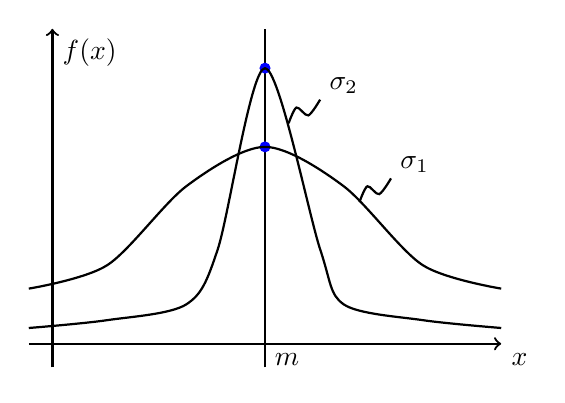
\begin{tikzpicture}
	\draw[thick,->] (0,0) -- (6,0) node[anchor=north west] {$x$};
	\draw[thick,->] (0.3,-0.3) -- (0.3,4) node[anchor=north west] {$f(x)$};

	\draw[thin,-] (3,-0.3) -- (3,4);
    \node[below right] at (3,0) {$m$};
	\fill[blue,thick] (3,3.5) circle (2pt);
	\fill[blue,thick] (3,2.5) circle (2pt);
	
	% \sigma_1
	\draw[thick] plot [smooth] coordinates 
	{(0,0.7) (1,1) (2, 2) (3,2.5) (4,2) (5,1) (6, 0.7)};
	\draw (4.9,2.5) node[anchor=north] {$\sigma_1$};
	\draw[thick] plot [smooth] coordinates {(4.2,1.8) (4.3,2) (4.45, 1.9) (4.6,2.1)};

	% \sigma_2
	\draw[thick] plot [smooth] coordinates 
	{(0,0.2) (1,0.3) (2, 0.5) (2.4, 1.2) (3,3.5) (3.7,1.2)  (4,0.5) (5,0.3) (6, 0.2)};
	\draw (4,3.5) node[anchor=north] {$\sigma_2$};
	\draw[thick] plot [smooth] coordinates {(3.3,2.8) (3.4,3) (3.55, 2.9) (3.7,3.1)};
\end{tikzpicture}

\ZAM Параметр $m$ характеризует положение центра симметрии графика $f(x)$. Параметр $\sigma$ отвечает за степень разброса значений случайной величины относительно среднего значения. Чем больше $\sigma$ тем больше разброс ($\sigma_1 > \sigma_2$)

Если $m=0,~\sigma=1$, то нормальная сл. вел. называется $X\sim N(0, 1)$ называется \B{стандартной} нормальной величиной, $f_{0,1}(x)=\tfrac{1}{\sqrt{2\pi}}e^{\tfrac{-x^2}{2}},x\in\R$

\ZAM Если нормальная сл. вел. не является стандартной:

$P\{a\leq x < b\}=\tfrac{1}{\sqrt{2\pi}\sigma}\intl_a^b e^{-\tfrac{(x-m)^2}{2\sigma^2}}dx=
\left| 
\begin{array}{l}
	t=\tfrac{x-m}{\sigma} \\
	dt=\tfrac{1}{\sigma}dx \\
	x=a\Rightarrow t=\tfrac{a-m}{\sigma}\\
	x=b\Rightarrow t=\tfrac{b-m}{\sigma} 
\end{array} 
\right| = \tfrac{\sigma}{\sqrt{2\pi}\sigma}\intl_{\tfrac{a-m}{\sigma}}^{\tfrac{b-m}{\sigma}}e^{-\tfrac{t^2}{2}}dt=$

$=\tfrac{1}{\sqrt{2\pi}}\intl_{\tfrac{a-m}{\sigma}}^{\tfrac{b-m}{\sigma}}e^{-\tfrac{t^2}{2}}dt=
\left| 
\begin{array}{l}
	\text{вероятность того, что} \\
	\text{станд. норм. случ. величина} \\
    \text{попала в } \left[\tfrac{a-m}{\sigma},~ \tfrac{b-m}{\sigma}\right) 
\end{array} 
\right| = \varPhi(\tfrac{b-m}{\sigma}) - \varPhi(\tfrac{a-m}{\sigma})$


\clearpage
